%%%%%%%%%%%%%%%%%%%%%%%%%%%%%%%%%%%%%%%%%%%%%%%%%%%%%%
% A Beamer template for University of Wollongong     %
% Based on THU beamer theme                          %
% Author: Qiuyu Lu                                   %
% Date: July 2024                                    %
% LPPL Licensed.                                     %
%%%%%%%%%%%%%%%%%%%%%%%%%%%%%%%%%%%%%%%%%%%%%%%%%%%%%%
% Customized for Sharif University of Technology     %
%%%%%%%%%%%%%%%%%%%%%%%%%%%%%%%%%%%%%%%%%%%%%%%%%%%%%%


\documentclass[serif, aspectratio=169]{beamer}
%\documentclass[serif]{beamer}  % for 4:3 ratio
\usepackage[T1]{fontenc} 
\usepackage{fourier} % see "http://faq.ktug.org/wiki/uploads/MathFonts.pdf" for other options
\usepackage{hyperref}
\usepackage{latexsym,amsmath,xcolor,multicol,booktabs,calligra}
\usepackage{graphicx,pstricks,listings,stackengine}
\usepackage{lipsum}
\usepackage{tikz}
\usetikzlibrary{positioning}
\usetikzlibrary{shapes.geometric} % Add this to include ellipse shapes
\usepackage{amsmath}
\usepackage{pgfplots}  % For plots
\usepackage{amsmath}   % For equations
\usepackage{array}     % For tables
\usepackage{url}
\pgfplotsset{compat=1.16}




\author{Ali Sharifi-Zarchi}
\title{Machine Learning (CE 40717)}
\subtitle{Fall 2024}
\institute{
    CE Department \\
    Sharif University of Technology
}
%\date{\small \today}
% \usepackage{UoWstyle}
\usepackage{SUTstyle}

% defs
\def\cmd#1{\texttt{\color{red}\footnotesize $\backslash$#1}}
\def\env#1{\texttt{\color{blue}\footnotesize #1}}
\definecolor{deepblue}{rgb}{0,0,0.5}
\definecolor{deepred}{RGB}{153,0,0}
\definecolor{deepgreen}{rgb}{0,0.5,0}
\definecolor{halfgray}{gray}{0.55}

\lstset{
    basicstyle=\ttfamily\small,
    keywordstyle=\bfseries\color{deepblue},
    emphstyle=\ttfamily\color{deepred},    % Custom highlighting style
    stringstyle=\color{deepgreen},
    numbers=left,
    numberstyle=\small\color{halfgray},
    rulesepcolor=\color{red!20!green!20!blue!20},
    frame=shadowbox,
}


\begin{document}

\begin{frame}
    \titlepage
    \vspace*{-0.6cm}
    \begin{figure}[htpb]
        \begin{center}
            \includegraphics[keepaspectratio, scale=0.25]{pic/sharif-main-logo.png}
        \end{center}
    \end{figure}
\end{frame}

\section{Gradient Descent}

\begin{frame}{How to Update Weights?}
    \begin{itemize}
        \item Imagine training a large model like ChatGPT. It has billions of parameters that need to be adjusted.
        \item If we used \textbf{random search} to update these weights, it would take an astronomical number of trials to find good parameters.
        \item How to make training feasible at this massive scale?
    \end{itemize}
    \begin{figure}[!htb]
  \begin{minipage}{0.3\textwidth}
     \centering
     \includegraphics[width=.9\linewidth]{pic/gd1.png}
  \end{minipage}\hfill
    \begin{minipage}{0.3\textwidth}
     \centering
     \includegraphics[width=.9\linewidth]{pic/gd2.png}
  \end{minipage}\hfill
  \begin{minipage}{0.3\textwidth}
     \centering
     \includegraphics[width=.9\linewidth]{pic/gd3.png}
  \end{minipage}
\end{figure}
\end{frame}

\begin{frame}{How to Update Weights?}
 \textbf{Options for Updating Weights:}
    \begin{itemize}
        \item \textbf{Random Search:} Tries values randomly—inefficient and impractical.
        \item \textcolor{green}{Gradient Descent:} Follows the slope of the loss function—efficient and guided.
    \end{itemize}
    
    \textbf{Why Gradient Descent?}
    \begin{itemize}
        \item It updates weights by following the slope, reducing error with each step.
        \item Controlled, stepwise updates ensure we move closer to minimizing the loss effectively.
    \end{itemize}
\end{frame}

\begin{frame}{How to Update Weights?}

    
    \begin{center}
        \includegraphics[width=10cm]{pic/ball.png}  
    \end{center}
\end{frame}

\begin{frame}{Gradient Descent: Concept and Weight Updates}
    \textbf{Gradient Descent}: Minimizes the loss function by updating weights based on the gradient.

    \textbf{Weight Update Rule}:
    \[
    w_{\text{new}} = w_{\text{old}} - \eta \cdot \frac{\partial L}{\partial w}
    \]
    Where:
    \begin{itemize}
        \item \( \eta \) is the learning rate (step size).
        \item \( \frac{\partial L}{\partial w} \) is the gradient of the loss function with respect to \( w \).
    \end{itemize}
\end{frame}

\begin{frame}{Example: Gradient Descent and Updating Weights}
    \textbf{Example Problem}:
    \begin{itemize}
        \item Initial weight: \( w_0 = 2 \)
        \item Learning rate: \( \eta = 0.1 \)
        \item Loss function: \( L(w) = (y - wx)^2 \)
    \end{itemize}
    
    \textbf{Gradient Calculation}:
    \[
    \frac{\partial L}{\partial w} = -2x(y - wx)
    \]
    
    \textbf{Example}: For \( x = 3 \), \( y = 10 \), and \( w_0 = 2 \),
    \[
    \frac{\partial L}{\partial w} = -36, \quad w_{\text{new}} = 5.6
    \]
\end{frame}

\begin{frame}{Gradient Descent: Formula and Process}
    \textbf{Weight Update Formula}:
    \[
    w_{\text{new}} = w_{\text{old}} - \eta \cdot \frac{\partial L}{\partial w}
    \]

    \textbf{Steps in Gradient Descent}:
    \begin{itemize}
        \item Compute the gradient of the loss function.
        \item Update the weights using the update rule.
        \item Repeat until convergence.
    \end{itemize}
    
    \vspace{-2cm} % Adjust vertical space to shift the text up
    \begin{flushright}
        \includegraphics[scale=0.3]{pic/GD.png} % Scale the image and place it to the Southeast
    \end{flushright}

\end{frame}


\section{Backpropagation}
\subsection{Forward and Backward Passes}
\begin{frame}{Example: One Neuron}
    \begin{figure}
        \vspace{-0.3cm}
        \includegraphics[width=.9\linewidth, height=\textheight, keepaspectratio]{pic/1.png}
    \end{figure}
\end{frame}

\begin{frame}{Forward Pass}
    \begin{figure}
        \vspace{-0.3cm}
        \includegraphics[width=.9\linewidth, height=\textheight, keepaspectratio]{pic/2.png}
    \end{figure}
\end{frame}

\begin{frame}{Backward Pass}
    \begin{figure}
        \vspace{-0.3cm}
        \includegraphics[width=.9\linewidth, height=\textheight, keepaspectratio]{pic/4.png}
    \end{figure}
\end{frame}


\begin{frame}{Backward Pass}
    \begin{figure}
        \vspace{-0.3cm}
        \includegraphics[width=.9\linewidth, height=\textheight, keepaspectratio]{pic/3.png}
    \end{figure}
\end{frame}

\begin{frame}{Backward Pass}
    \begin{figure}
        \vspace{-0.3cm}
        \includegraphics[width=.9\linewidth, height=\textheight, keepaspectratio]{pic/5.png}
    \end{figure}
\end{frame}

\begin{frame}{Backpropagation: a simple example}
        % Start of the columns environment
    \begin{columns}
       
        % Left column: Steps with equations
        \begin{column}{0.4\textwidth}
            \vspace{-0.4cm} % Added 'cm' as a unit
            \textbf{Function:} 
            \[
            f(x, y, z) = (x + y)z
            \]
            
        \end{column}

        % Right column: Computational graph (TikZ diagram)
        \begin{column}{0.6\textwidth}
            \begin{center}
            \begin{tikzpicture}[scale=0.9, every node/.style={scale=0.8}]
                
                % Nodes
                \node at (0,0) (x) {\(x = -2\)};
                \node at (0,-1.5) (y) {\(y = 5\)};
                \node at (2,-0.75) (sum) [draw, circle] {\(+\)};
                \node at (3.5,-0.75) (q) {\(q = 3\)};
                \node at (5,-2) (z) {\(z = -4\)};
                \node at (7,-1) (mult) [draw, circle] {\(\times\)};
                \node at (8.5,-1) (f) {\(f = -12\)};

                % Arrows
                \draw[->] (x) -- (sum);
                \draw[->] (y) -- (sum);
                \draw[->] (sum) -- (q);
                \draw[->] (q) -- (mult);
                \draw[->] (z) -- (mult);
                \draw[->] (mult) -- (f);
            \end{tikzpicture}
            \end{center}
        \end{column}

    \end{columns}
\end{frame}


\begin{frame}{Backpropagation: a simple example}
        % Start of the columns environment
    \begin{columns}
       
        % Left column: Steps with equations
        \begin{column}{0.4\textwidth}
            \vspace{-0.4cm}
            \textbf{Function:} 
            \[
            f(x, y, z) = (x + y)z
            \]
            \textbf{Example:} 
            \[
            x = -2, \quad y = 5, \quad z = -4
            \]
        \end{column}

        % Right column: Computational graph (TikZ diagram)
        \begin{column}{0.6\textwidth}
            \begin{center}
            \begin{tikzpicture}[scale=0.9, every node/.style={scale=0.8}]
                
                % Nodes
                \node at (0,0) (x) {\(x = -2\)};
                \node at (0,-1.5) (y) {\(y = 5\)};
                \node at (2,-0.75) (sum) [draw, circle] {\(+\)};
                \node at (3.5,-0.75) (q) {\(q = 3\)};
                \node at (5,-2) (z) {\(z = -4\)};
                \node at (7,-1) (mult) [draw, circle] {\(\times\)};
                \node at (8.5,-1) (f) {\(f = -12\)};

                % Arrows
                \draw[->] (x) -- (sum);
                \draw[->] (y) -- (sum);
                \draw[->] (sum) -- (q);
                \draw[->] (q) -- (mult);
                \draw[->] (z) -- (mult);
                \draw[->] (mult) -- (f);
            \end{tikzpicture}
            \end{center}
        \end{column}

    \end{columns}
\end{frame}

\begin{frame}{Backpropagation: a simple example}
        % Start of the columns environment
    \begin{columns}
       
        % Left column: Steps with equations
        \begin{column}{0.4\textwidth}
            \vspace{-0.4cm}
            \textbf{Function:} 
            \[
            f(x, y, z) = (x + y)z
            \]
            \textbf{Example:} 
            \[
            x = -2, \quad y = 5, \quad z = -4
            \]
            
            % Step 1
            \textcolor{green}{\textbf{Step 1:}}
            \[
             q = x + y, \quad
            \frac{\partial q}{\partial x} = 1, \quad \frac{\partial q}{\partial y} = 1
            \]
        \end{column}

        % Right column: Computational graph (TikZ diagram)
        \begin{column}{0.6\textwidth}
            \begin{center}
            \begin{tikzpicture}[scale=0.9, every node/.style={scale=0.8}]
                
                % Nodes
                \node at (0,0) (x) {\(x = -2\)};
                \node at (0,-1.5) (y) {\(y = 5\)};
                \node at (2,-0.75) (sum) [draw, circle] {\(+\)};
                \node at (3.5,-0.75) (q) {\(q = 3\)};
                \node at (5,-2) (z) {\(z = -4\)};
                \node at (7,-1) (mult) [draw, circle] {\(\times\)};
                \node at (8.5,-1) (f) {\(f = -12\)};

                % Arrows
                \draw[->] (x) -- (sum);
                \draw[->] (y) -- (sum);
                \draw[->] (sum) -- (q);
                \draw[->] (q) -- (mult);
                \draw[->] (z) -- (mult);
                \draw[->] (mult) -- (f);
            \end{tikzpicture}
            \end{center}
        \end{column}

    \end{columns}
\end{frame}

\begin{frame}{Backpropagation: a simple example}
        % Start of the columns environment
    \begin{columns}
       
        % Left column: Steps with equations
        \begin{column}{0.4\textwidth}
            \vspace{-0.4cm}
            \textbf{Function:} 
            \[
            f(x, y, z) = (x + y)z
            \]
            \textbf{Example:} 
            \[
            x = -2, \quad y = 5, \quad z = -4
            \]
            
            % Step 1
            \textcolor{green}{\textbf{Step 1:}}
            \[
             q = x + y, \quad
            \frac{\partial q}{\partial x} = 1, \quad \frac{\partial q}{\partial y} = 1
            \]
            
            % Step 2
            \textcolor{green}{\textbf{Step 2:}}

            \[
            f = qz, \quad
            \frac{\partial f}{\partial q} = z, \quad \frac{\partial f}{\partial z} = q
            \]
        \end{column}

        % Right column: Computational graph (TikZ diagram)
        \begin{column}{0.6\textwidth}
            \begin{center}
            \begin{tikzpicture}[scale=0.9, every node/.style={scale=0.8}]
                
                % Nodes
                \node at (0,0) (x) {\(x = -2\)};
                \node at (0,-1.5) (y) {\(y = 5\)};
                \node at (2,-0.75) (sum) [draw, circle] {\(+\)};
                \node at (3.5,-0.75) (q) {\(q = 3\)};
                \node at (5,-2) (z) {\(z = -4\)};
                \node at (7,-1) (mult) [draw, circle] {\(\times\)};
                \node at (8.5,-1) (f) {\(f = -12\)};

                % Arrows
                \draw[->] (x) -- (sum);
                \draw[->] (y) -- (sum);
                \draw[->] (sum) -- (q);
                \draw[->] (q) -- (mult);
                \draw[->] (z) -- (mult);
                \draw[->] (mult) -- (f);
            \end{tikzpicture}
            \end{center}
        \end{column}
    \end{columns}
\end{frame}

\begin{frame}{Backpropagation: a simple example}
        % Start of the columns environment
    \begin{columns}
       
        % Left column: Steps with equations
        \begin{column}{0.4\textwidth}
            \vspace{-0.4cm}
            \textbf{Function:} 
            \[
            f(x, y, z) = (x + y)z
            \]
            \textbf{Example:} 
            \[
            x = -2, \quad y = 5, \quad z = -4
            \]
            
            % Step 1
            \textcolor{green}{\textbf{Step 1:}}
            \[
             q = x + y, \quad
            \frac{\partial q}{\partial x} = 1, \quad \frac{\partial q}{\partial y} = 1
            \]
            
            % Step 2
            \textcolor{green}{\textbf{Step 2:}}

            \[
            f = qz, \quad
            \frac{\partial f}{\partial q} = z, \quad \frac{\partial f}{\partial z} = q
            \]
        \end{column}

        % Right column: Computational graph (TikZ diagram)
        \begin{column}{0.6\textwidth}
            \begin{center}
            \begin{tikzpicture}[scale=0.9, every node/.style={scale=0.8}]
                
                % Nodes
                \node at (0,0) (x) {\(x = -2\)};
                \node at (0,-1.5) (y) {\(y = 5\)};
                \node at (2,-0.75) (sum) [draw, circle] {\(+\)};
                \node at (3.5,-0.75) (q) {\(q = 3\)};
                \node at (5,-2) (z) {\(z = -4\)};
                \node at (7,-1) (mult) [draw, circle] {\(\times\)};
                \node at (8.5,-1) (f) {\(f = -12\)};

                % Arrows
                \draw[->] (x) -- (sum);
                \draw[->] (y) -- (sum);
                \draw[->] (sum) -- (q);
                \draw[->] (q) -- (mult);
                \draw[->] (z) -- (mult);
                \draw[->] (mult) -- (f);
            \end{tikzpicture}
            \end{center}
            \textcolor{red}{ 
            \[
            want \quad
            \frac{\partial f}{\partial x}, \quad \frac{\partial f}{\partial y}, \quad
            \frac{\partial f}{\partial z}
            \] 
            }
        \end{column}
    \end{columns}
\end{frame}

\begin{frame}{Backpropagation: a simple example}

    % Start of the columns environment
    \begin{columns}
       
        % Left column: Steps with equations
        \begin{column}{0.4\textwidth}
            \vspace{-0.4cm}
            \textbf{Function:} 
            \[
            f(x, y, z) = (x + y)z
            \]
            \textbf{Example:} 
            \[
            x = -2, \quad y = 5, \quad z = -4
            \]
            
            % Step 1
            \textcolor{green}{\textbf{Step 1:}}
            \[
             q = x + y, \quad
            \frac{\partial q}{\partial x} = 1, \quad \frac{\partial q}{\partial y} = 1
            \]
            
            % Step 2
            \textcolor{green}{\textbf{Step 2:}}

            \[
            f = qz, \quad
            \frac{\partial f}{\partial q} = z, \quad \frac{\partial f}{\partial z} = q
            \]
        \end{column}

        % Right column: Computational graph (TikZ diagram)
        \begin{column}{0.6\textwidth}
            \begin{center}
            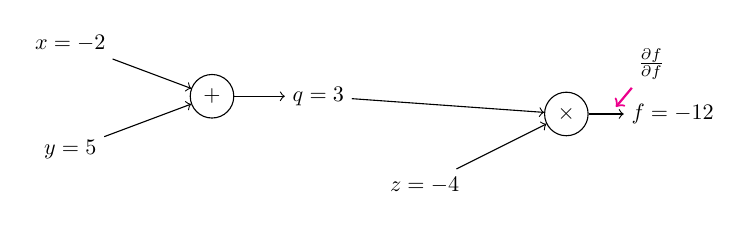
\begin{tikzpicture}[scale=0.9, every node/.style={scale=0.8}]
                
                % Nodes
                \node at (0,0) (x) {\(x = -2\)};
                \node at (0,-1.5) (y) {\(y = 5\)};
                \node at (2,-0.75) (sum) [draw, circle] {\(+\)};
                \node at (3.5,-0.75) (q) {\(q = 3\)};
                \node at (5,-2) (z) {\(z = -4\)};
                \node at (7,-1) (mult) [draw, circle] {\(\times\)};
                \node at (8.5,-1) (f) {\(f = -12\)};

                % Arrows
                \draw[->] (x) -- (sum);
                \draw[->] (y) -- (sum);
                \draw[->] (sum) -- (q);
                \draw[->] (q) -- (mult);
                \draw[->] (z) -- (mult);
                \draw[->] (mult) -- (f);

                % Pink Element: Arrow and Derivative (df/df)
                \node at (8.2,-0.3) (dfdf_text) {\(\frac{\partial f}{\partial f}\)};
                \draw[->, thick, magenta] (dfdf_text) -- (7.7,-0.9);

            \end{tikzpicture}
            \end{center}
            \textcolor{red}{ 
            \[
            want \quad
            \frac{\partial f}{\partial x}, \quad \frac{\partial f}{\partial y}, \quad
            \frac{\partial f}{\partial z}
            \] 
            }
        \end{column}

    \end{columns}

\end{frame}

\begin{frame}{Backpropagation: a simple example}

    % Start of the columns environment
    \begin{columns}
       
        % Left column: Steps with equations
        \begin{column}{0.4\textwidth}
            \vspace{-0.4cm}
            \textbf{Function:} 
            \[
            f(x, y, z) = (x + y)z
            \]
            \textbf{Example:} 
            \[
            x = -2, \quad y = 5, \quad z = -4
            \]
            
            % Step 1
            \textcolor{green}{\textbf{Step 1:}}
            \[
             q = x + y, \quad
            \frac{\partial q}{\partial x} = 1, \quad \frac{\partial q}{\partial y} = 1
            \]
            
            % Step 2
            \textcolor{green}{\textbf{Step 2:}}

            \[
            f = qz, \quad
            \frac{\partial f}{\partial q} = z, \quad \frac{\partial f}{\partial z} = q
            \]
        \end{column}

        % Right column: Computational graph (TikZ diagram)
        \begin{column}{0.6\textwidth}
            \begin{center}
            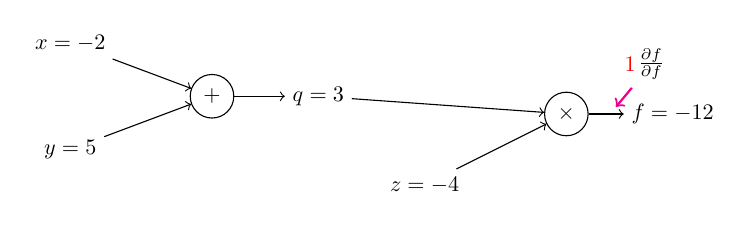
\begin{tikzpicture}[scale=0.9, every node/.style={scale=0.8}]
                
                % Nodes
                \node at (0,0) (x) {\(x = -2\)};
                \node at (0,-1.5) (y) {\(y = 5\)};
                \node at (2,-0.75) (sum) [draw, circle] {\(+\)};
                \node at (3.5,-0.75) (q) {\(q = 3\)};
                \node at (5,-2) (z) {\(z = -4\)};
                \node at (7,-1) (mult) [draw, circle] {\(\times\)};
                \node at (8.5,-1) (f) {\(f = -12\)};
                \textcolor{red}{\node at (7.9,-0.3) (one) {\(1\)};}  % 

                % Arrows
                \draw[->] (x) -- (sum);
                \draw[->] (y) -- (sum);
                \draw[->] (sum) -- (q);
                \draw[->] (q) -- (mult);
                \draw[->] (z) -- (mult);
                \draw[->] (mult) -- (f);

                % Pink Element: Arrow and Derivative (df/df)
                \node at (8.2,-0.3) (dfdf_text) {\(\frac{\partial f}{\partial f}\)};
                \draw[->, thick, magenta] (dfdf_text) -- (7.7,-0.9);

            \end{tikzpicture}
            \end{center}
            \textcolor{red}{ 
            \[
            want \quad
            \frac{\partial f}{\partial x}, \quad \frac{\partial f}{\partial y}, \quad
            \frac{\partial f}{\partial z}
            \] 
            }
        \end{column}

    \end{columns}

\end{frame}

\begin{frame}{Backpropagation: a simple example}

    % Start of the columns environment
    \begin{columns}
       
        % Left column: Steps with equations
        \begin{column}{0.4\textwidth}
            \vspace{-0.4cm}
            \textbf{Function:} 
            \[
            f(x, y, z) = (x + y)z
            \]
            \textbf{Example:} 
            \[
            x = -2, \quad y = 5, \quad z = -4
            \]
            
            % Step 1
            \textcolor{green}{\textbf{Step 1:}}
            \[
             q = x + y, \quad
            \frac{\partial q}{\partial x} = 1, \quad \frac{\partial q}{\partial y} = 1
            \]
            
            % Step 2
            \textcolor{green}{\textbf{Step 2:}}

            \[
            f = qz, \quad
            \frac{\partial f}{\partial q} = z, \quad \frac{\partial f}{\partial z} = q
            \]
        \end{column}

        % Right column: Computational graph (TikZ diagram)
        \begin{column}{0.6\textwidth}
            \begin{center}
            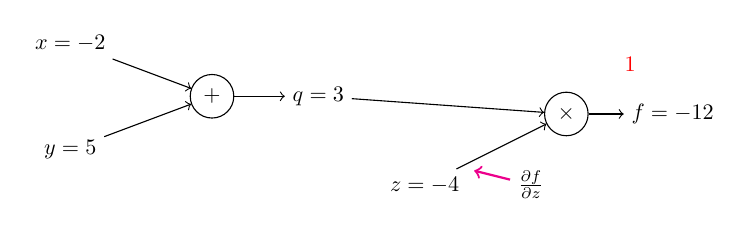
\begin{tikzpicture}[scale=0.9, every node/.style={scale=0.8}]
                
                % Nodes
                \node at (0,0) (x) {\(x = -2\)};
                \node at (0,-1.5) (y) {\(y = 5\)};
                \node at (2,-0.75) (sum) [draw, circle] {\(+\)};
                \node at (3.5,-0.75) (q) {\(q = 3\)};
                \node at (5,-2) (z) {\(z = -4\)};
                \node at (7,-1) (mult) [draw, circle] {\(\times\)};
                \node at (8.5,-1) (f) {\(f = -12\)};
                \textcolor{red}{\node at (7.9,-0.3) (one) {\(1\)};} 

                % Arrows
                \draw[->] (x) -- (sum);
                \draw[->] (y) -- (sum);
                \draw[->] (sum) -- (q);
                \draw[->] (q) -- (mult);
                \draw[->] (z) -- (mult);
                \draw[->] (mult) -- (f);

                % Pink Element for df/dz: Add arrow and derivative box
                \node at (6.5, -2) (dfdz_text) {\(\frac{\partial f}{\partial z}\)};
                \draw[->, thick, magenta] (dfdz_text) -- (5.7, -1.8);  % Arrow pointing from the text to z = -4


            \end{tikzpicture}
            \end{center}
            \textcolor{red}{ 
            \[
            want \quad
            \frac{\partial f}{\partial x}, \quad \frac{\partial f}{\partial y}, \quad
            \frac{\partial f}{\partial z}
            \] 
            }
        \end{column}

    \end{columns}

\end{frame}

\begin{frame}{Backpropagation: a simple example}

    % Start of the columns environment
    \begin{columns}
       
        % Left column: Steps with equations
        \begin{column}{0.4\textwidth}
            \vspace{-0.4cm}
            \textbf{Function:} 
            \[
            f(x, y, z) = (x + y)z
            \]
            \textbf{Example:} 
            \[
            x = -2, \quad y = 5, \quad z = -4
            \]
            
            % Step 1
            \textcolor{green}{\textbf{Step 1:}}
            \[
             q = x + y, \quad
            \frac{\partial q}{\partial x} = 1, \quad \frac{\partial q}{\partial y} = 1
            \]
            
            % Step 2
            \textcolor{green}{\textbf{Step 2:}}

            \[
            f = qz, \quad
            \frac{\partial f}{\partial q} = z, \quad \frac{\partial f}{\partial z} = q
            \]
        \end{column}

        % Right column: Computational graph (TikZ diagram)
        \begin{column}{0.6\textwidth}
            \begin{center}
            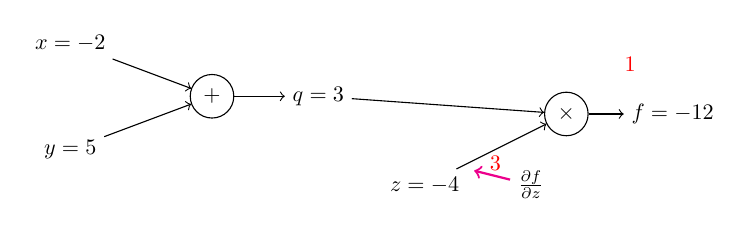
\begin{tikzpicture}[scale=0.9, every node/.style={scale=0.8}]
                
                % Nodes
                \node at (0,0) (x) {\(x = -2\)};
                \node at (0,-1.5) (y) {\(y = 5\)};
                \node at (2,-0.75) (sum) [draw, circle] {\(+\)};
                \node at (3.5,-0.75) (q) {\(q = 3\)};
                \node at (5,-2) (z) {\(z = -4\)};
                \node at (7,-1) (mult) [draw, circle] {\(\times\)};
                \node at (8.5,-1) (f) {\(f = -12\)};
                \textcolor{red}{\node at (7.9,-0.3) (one) {\(1\)};} 
                \textcolor{red}{\node at (6,-1.7) (three) {\(3\)};} 

                % Arrows
                \draw[->] (x) -- (sum);
                \draw[->] (y) -- (sum);
                \draw[->] (sum) -- (q);
                \draw[->] (q) -- (mult);
                \draw[->] (z) -- (mult);
                \draw[->] (mult) -- (f);

                % Pink Element for df/dz: Add arrow and derivative box
                \node at (6.5, -2) (dfdz_text) {\(\frac{\partial f}{\partial z}\)};
                \draw[->, thick, magenta] (dfdz_text) -- (5.7, -1.8);  % Arrow pointing from the text to z = -4


            \end{tikzpicture}
            \end{center}
            \textcolor{red}{ 
            \[
            want \quad
            \frac{\partial f}{\partial x}, \quad \frac{\partial f}{\partial y}, \quad
            \frac{\partial f}{\partial z}
            \] 
            }
        \end{column}

    \end{columns}

\end{frame}

\begin{frame}{Backpropagation: a simple example}

    % Start of the columns environment
    \begin{columns}
       
        % Left column: Steps with equations
        \begin{column}{0.4\textwidth}
            \vspace{-0.4cm}
            \textbf{Function:} 
            \[
            f(x, y, z) = (x + y)z
            \]
            \textbf{Example:} 
            \[
            x = -2, \quad y = 5, \quad z = -4
            \]
            
            % Step 1
            \textcolor{green}{\textbf{Step 1:}}
            \[
             q = x + y, \quad
            \frac{\partial q}{\partial x} = 1, \quad \frac{\partial q}{\partial y} = 1
            \]
            
            % Step 2
            \textcolor{green}{\textbf{Step 2:}}

            \[
            f = qz, \quad
            \frac{\partial f}{\partial q} = z, \quad \frac{\partial f}{\partial z} = q
            \]
        \end{column}

        % Right column: Computational graph (TikZ diagram)
        \begin{column}{0.6\textwidth}
            \begin{center}
            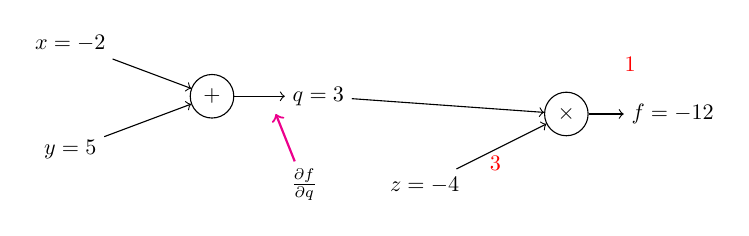
\begin{tikzpicture}[scale=0.9, every node/.style={scale=0.8}]
                
                % Nodes
                \node at (0,0) (x) {\(x = -2\)};
                \node at (0,-1.5) (y) {\(y = 5\)};
                \node at (2,-0.75) (sum) [draw, circle] {\(+\)};
                \node at (3.5,-0.75) (q) {\(q = 3\)};
                \node at (5,-2) (z) {\(z = -4\)};
                \node at (7,-1) (mult) [draw, circle] {\(\times\)};
                \node at (8.5,-1) (f) {\(f = -12\)};
                \textcolor{red}{\node at (7.9,-0.3) (one) {\(1\)};} 
                \textcolor{red}{\node at (6,-1.7) (three) {\(3\)};} 

                % Arrows
                \draw[->] (x) -- (sum);
                \draw[->] (y) -- (sum);
                \draw[->] (sum) -- (q);
                \draw[->] (q) -- (mult);
                \draw[->] (z) -- (mult);
                \draw[->] (mult) -- (f);

                % Pink Element for df/dz: Add arrow and derivative box
                \node at (3.3, -2) (dfdz_text) {\(\frac{\partial f}{\partial q}\)};
                \draw[->, thick, magenta] (dfdz_text) -- (2.9, -1); 


            \end{tikzpicture}
            \end{center}
            \textcolor{red}{ 
            \[
            want \quad
            \frac{\partial f}{\partial x}, \quad \frac{\partial f}{\partial y}, \quad
            \frac{\partial f}{\partial z}
            \] 
            }
        \end{column}

    \end{columns}

\end{frame}
\begin{frame}{Backpropagation: a simple example}

    % Start of the columns environment
    \begin{columns}
       
        % Left column: Steps with equations
        \begin{column}{0.4\textwidth}
            \vspace{-0.4cm}
            \textbf{Function:} 
            \[
            f(x, y, z) = (x + y)z
            \]
            \textbf{Example:} 
            \[
            x = -2, \quad y = 5, \quad z = -4
            \]
            
            % Step 1
            \textcolor{green}{\textbf{Step 1:}}
            \[
             q = x + y, \quad
            \frac{\partial q}{\partial x} = 1, \quad \frac{\partial q}{\partial y} = 1
            \]
            
            % Step 2
            \textcolor{green}{\textbf{Step 2:}}

            \[
            f = qz, \quad
            \frac{\partial f}{\partial q} = z, \quad \frac{\partial f}{\partial z} = q
            \]
        \end{column}

        % Right column: Computational graph (TikZ diagram)
        \begin{column}{0.6\textwidth}
            \begin{center}
            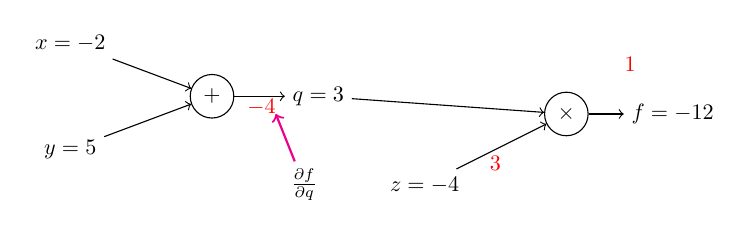
\begin{tikzpicture}[scale=0.9, every node/.style={scale=0.8}]
                
                % Nodes
                \node at (0,0) (x) {\(x = -2\)};
                \node at (0,-1.5) (y) {\(y = 5\)};
                \node at (2,-0.75) (sum) [draw, circle] {\(+\)};
                \node at (3.5,-0.75) (q) {\(q = 3\)};
                \node at (5,-2) (z) {\(z = -4\)};
                \node at (7,-1) (mult) [draw, circle] {\(\times\)};
                \node at (8.5,-1) (f) {\(f = -12\)};
                \textcolor{red}{\node at (7.9,-0.3) (one) {\(1\)};} 
                \textcolor{red}{\node at (6,-1.7) (three) {\(3\)};} 
                \textcolor{red}{\node at (2.7,-0.9) (minus four) {\(-4\)};} 

                % Arrows
                \draw[->] (x) -- (sum);
                \draw[->] (y) -- (sum);
                \draw[->] (sum) -- (q);
                \draw[->] (q) -- (mult);
                \draw[->] (z) -- (mult);
                \draw[->] (mult) -- (f);

                % Pink Element for df/dz: Add arrow and derivative box
                \node at (3.3, -2) (dfdz_text) {\(\frac{\partial f}{\partial q}\)};
                \draw[->, thick, magenta] (dfdz_text) -- (2.9, -1); 


            \end{tikzpicture}
            \end{center}
            \textcolor{red}{ 
            \[
            want \quad
            \frac{\partial f}{\partial x}, \quad \frac{\partial f}{\partial y}, \quad
            \frac{\partial f}{\partial z}
            \] 
            }
        \end{column}

    \end{columns}

\end{frame}

\begin{frame}{Backpropagation: a simple example}

    % Start of the columns environment
    \begin{columns}
       
        % Left column: Steps with equations
        \begin{column}{0.4\textwidth}
            \vspace{-0.4cm}
            \textbf{Function:} 
            \[
            f(x, y, z) = (x + y)z
            \]
            \textbf{Example:} 
            \[
            x = -2, \quad y = 5, \quad z = -4
            \]
            
            % Step 1
            \textcolor{green}{\textbf{Step 1:}}
            \[
             q = x + y, \quad
            \frac{\partial q}{\partial x} = 1, \quad \frac{\partial q}{\partial y} = 1
            \]
            
            % Step 2
            \textcolor{green}{\textbf{Step 2:}}

            \[
            f = qz, \quad
            \frac{\partial f}{\partial q} = z, \quad \frac{\partial f}{\partial z} = q
            \]
        \end{column}

        % Right column: Computational graph (TikZ diagram)
        \begin{column}{0.6\textwidth}
            \begin{center}
            \begin{tikzpicture}[scale=0.9, every node/.style={scale=0.8}]
                
                % Nodes
                \node at (0,0) (x) {\(x = -2\)};
                \node at (0,-1.5) (y) {\(y = 5\)};
                \node at (2,-0.75) (sum) [draw, circle] {\(+\)};
                \node at (3.5,-0.75) (q) {\(q = 3\)};
                \node at (5,-2) (z) {\(z = -4\)};
                \node at (7,-1) (mult) [draw, circle] {\(\times\)};
                \node at (8.5,-1) (f) {\(f = -12\)};
                \textcolor{red}{\node at (7.9,-0.3) (one) {\(1\)};} 
                \textcolor{red}{\node at (6,-1.7) (three) {\(3\)};} 
                \textcolor{red}{\node at (2.7,-0.9) (minus four) {\(-4\)};} 
                

                % Arrows
                \draw[->] (x) -- (sum);
                \draw[->] (y) -- (sum);
                \draw[->] (sum) -- (q);
                \draw[->] (q) -- (mult);
                \draw[->] (z) -- (mult);
                \draw[->] (mult) -- (f);

                % Pink Element for df/dz: Add arrow and derivative box
                \node at (1.5, -2.5) (dfdz_text) {\(\frac{\partial f}{\partial y}\)};
                \draw[->, thick, magenta] (dfdz_text) -- (1, -1.5); 

            \end{tikzpicture}
            \end{center}
            
            \[
            \textcolor{red}{ 
            want \quad
            \frac{\partial f}{\partial x}, \quad \frac{\partial f}{\partial y}, \quad
            \frac{\partial f}{\partial z}, \quad
            }
            Chain\quad rule \quad
            \frac{\partial f}{\partial y} =  \frac{\partial f}{\partial q}
            \frac{\partial q}{\partial y}
            \] 
            
        \end{column}

    \end{columns}

\end{frame}

\begin{frame}{Backpropagation: a simple example}

    % Start of the columns environment
    \begin{columns}
       
        % Left column: Steps with equations
        \begin{column}{0.4\textwidth}
            \vspace{-0.4cm}
            \textbf{Function:} 
            \[
            f(x, y, z) = (x + y)z
            \]
            \textbf{Example:} 
            \[
            x = -2, \quad y = 5, \quad z = -4
            \]
            
            % Step 1
            \textcolor{green}{\textbf{Step 1:}}
            \[
             q = x + y, \quad
            \frac{\partial q}{\partial x} = 1, \quad \frac{\partial q}{\partial y} = 1
            \]
            
            % Step 2
            \textcolor{green}{\textbf{Step 2:}}

            \[
            f = qz, \quad
            \frac{\partial f}{\partial q} = z, \quad \frac{\partial f}{\partial z} = q
            \]
        \end{column}

        % Right column: Computational graph (TikZ diagram)
        \begin{column}{0.6\textwidth}
            \begin{center}
            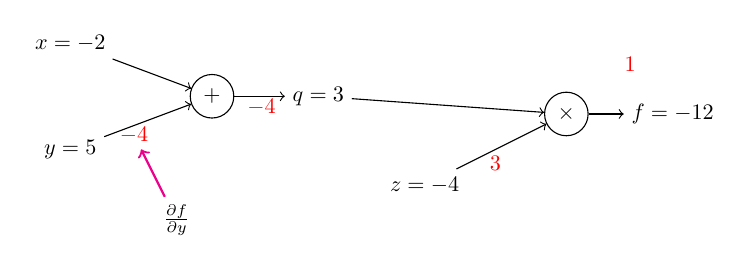
\begin{tikzpicture}[scale=0.9, every node/.style={scale=0.8}]
                
                % Nodes
                \node at (0,0) (x) {\(x = -2\)};
                \node at (0,-1.5) (y) {\(y = 5\)};
                \node at (2,-0.75) (sum) [draw, circle] {\(+\)};
                \node at (3.5,-0.75) (q) {\(q = 3\)};
                \node at (5,-2) (z) {\(z = -4\)};
                \node at (7,-1) (mult) [draw, circle] {\(\times\)};
                \node at (8.5,-1) (f) {\(f = -12\)};
                \textcolor{red}{\node at (7.9,-0.3) (one) {\(1\)};} 
                \textcolor{red}{\node at (6,-1.7) (three) {\(3\)};} 
                \textcolor{red}{\node at (2.7,-0.9) (minus four) {\(-4\)};} 
                \textcolor{red}{\node at (0.9,-1.3) (minus four) {\(-4\)};} 
                

                % Arrows
                \draw[->] (x) -- (sum);
                \draw[->] (y) -- (sum);
                \draw[->] (sum) -- (q);
                \draw[->] (q) -- (mult);
                \draw[->] (z) -- (mult);
                \draw[->] (mult) -- (f);

                % Pink Element for df/dz: Add arrow and derivative box
                \node at (1.5, -2.5) (dfdz_text) {\(\frac{\partial f}{\partial y}\)};
                \draw[->, thick, magenta] (dfdz_text) -- (1, -1.5); 

            \end{tikzpicture}
            \end{center}
            
            \[
            \textcolor{red}{ 
            want \quad
            \frac{\partial f}{\partial x}, \quad \frac{\partial f}{\partial y}, \quad
            \frac{\partial f}{\partial z}, \quad
            }
            Chain\quad rule \quad
            \frac{\partial f}{\partial y} =  \frac{\partial f}{\partial q}
            \frac{\partial q}{\partial y}
            \] 
            
        \end{column}

    \end{columns}

\end{frame}

\begin{frame}{Backpropagation: a simple example}

    % Start of the columns environment
    \begin{columns}
       
        % Left column: Steps with equations
        \begin{column}{0.4\textwidth}
            \vspace{-0.4cm}
            \textbf{Function:} 
            \[
            f(x, y, z) = (x + y)z
            \]
            \textbf{Example:} 
            \[
            x = -2, \quad y = 5, \quad z = -4
            \]
            
            % Step 1
            \textcolor{green}{\textbf{Step 1:}}
            \[
             q = x + y, \quad
            \frac{\partial q}{\partial x} = 1, \quad \frac{\partial q}{\partial y} = 1
            \]
            
            % Step 2
            \textcolor{green}{\textbf{Step 2:}}

            \[
            f = qz, \quad
            \frac{\partial f}{\partial q} = z, \quad \frac{\partial f}{\partial z} = q
            \]
        \end{column}

        % Right column: Computational graph (TikZ diagram)
        \begin{column}{0.6\textwidth}
            \begin{center}
            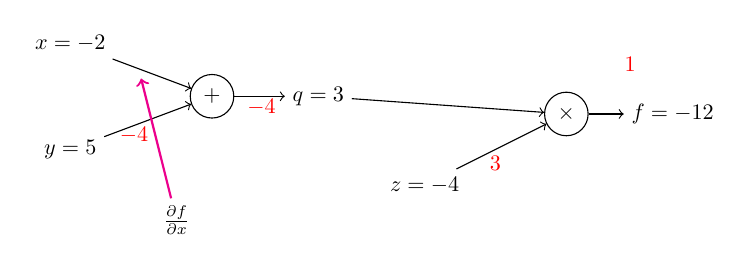
\begin{tikzpicture}[scale=0.9, every node/.style={scale=0.8}]
                
                % Nodes
                \node at (0,0) (x) {\(x = -2\)};
                \node at (0,-1.5) (y) {\(y = 5\)};
                \node at (2,-0.75) (sum) [draw, circle] {\(+\)};
                \node at (3.5,-0.75) (q) {\(q = 3\)};
                \node at (5,-2) (z) {\(z = -4\)};
                \node at (7,-1) (mult) [draw, circle] {\(\times\)};
                \node at (8.5,-1) (f) {\(f = -12\)};
                \textcolor{red}{\node at (7.9,-0.3) (one) {\(1\)};} 
                \textcolor{red}{\node at (6,-1.7) (three) {\(3\)};} 
                \textcolor{red}{\node at (2.7,-0.9) (minus four) {\(-4\)};} 
                \textcolor{red}{\node at (0.9,-1.3) (minus four) {\(-4\)};} 

                

                % Arrows
                \draw[->] (x) -- (sum);
                \draw[->] (y) -- (sum);
                \draw[->] (sum) -- (q);
                \draw[->] (q) -- (mult);
                \draw[->] (z) -- (mult);
                \draw[->] (mult) -- (f);

                % Pink Element for df/dz: Add arrow and derivative box
                \node at (1.5, -2.5) (dfdz_text) {\(\frac{\partial f}{\partial x}\)};
                \draw[->, thick, magenta] (dfdz_text) -- (1, -0.5); 

            \end{tikzpicture}
            \end{center}
            
            \[
            \textcolor{red}{ 
            want \quad
            \frac{\partial f}{\partial x}, \quad \frac{\partial f}{\partial y}, \quad
            \frac{\partial f}{\partial z}, \quad
            }
            Chain\quad rule \quad
            \frac{\partial f}{\partial x} =  \frac{\partial f}{\partial q}
            \frac{\partial q}{\partial x}
            \] 
            
        \end{column}

    \end{columns}

\end{frame}
\begin{frame}{Backpropagation: a simple example}

    % Start of the columns environment
    \begin{columns}
       
        % Left column: Steps with equations
        \begin{column}{0.4\textwidth}
            \vspace{-0.4cm}
            \textbf{Function:} 
            \[
            f(x, y, z) = (x + y)z
            \]
            \textbf{Example:} 
            \[
            x = -2, \quad y = 5, \quad z = -4
            \]
            
            % Step 1
            \textcolor{green}{\textbf{Step 1:}}
            \[
             q = x + y, \quad
            \frac{\partial q}{\partial x} = 1, \quad \frac{\partial q}{\partial y} = 1
            \]
            
            % Step 2
            \textcolor{green}{\textbf{Step 2:}}

            \[
            f = qz, \quad
            \frac{\partial f}{\partial q} = z, \quad \frac{\partial f}{\partial z} = q
            \]
        \end{column}

        % Right column: Computational graph (TikZ diagram)
        \begin{column}{0.6\textwidth}
            \begin{center}
            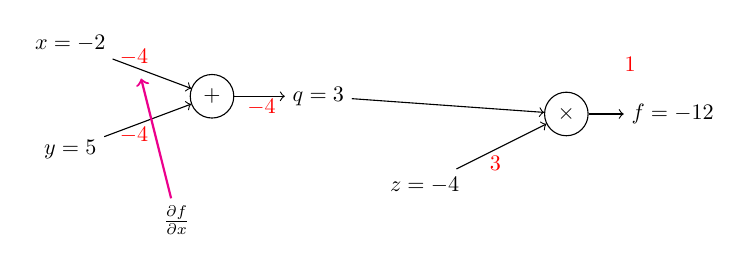
\begin{tikzpicture}[scale=0.9, every node/.style={scale=0.8}]
                
                % Nodes
                \node at (0,0) (x) {\(x = -2\)};
                \node at (0,-1.5) (y) {\(y = 5\)};
                \node at (2,-0.75) (sum) [draw, circle] {\(+\)};
                \node at (3.5,-0.75) (q) {\(q = 3\)};
                \node at (5,-2) (z) {\(z = -4\)};
                \node at (7,-1) (mult) [draw, circle] {\(\times\)};
                \node at (8.5,-1) (f) {\(f = -12\)};
                \textcolor{red}{\node at (7.9,-0.3) (one) {\(1\)};} 
                \textcolor{red}{\node at (6,-1.7) (three) {\(3\)};} 
                \textcolor{red}{\node at (2.7,-0.9) (minus four) {\(-4\)};} 
                \textcolor{red}{\node at (0.9,-0.2) (minus four) {\(-4\)};} 
                \textcolor{red}{\node at (0.9,-1.3) (minus four) {\(-4\)};} 

                % Arrows
                \draw[->] (x) -- (sum);
                \draw[->] (y) -- (sum);
                \draw[->] (sum) -- (q);
                \draw[->] (q) -- (mult);
                \draw[->] (z) -- (mult);
                \draw[->] (mult) -- (f);

                % Pink Element for df/dz: Add arrow and derivative box
                \node at (1.5, -2.5) (dfdz_text) {\(\frac{\partial f}{\partial x}\)};
                \draw[->, thick, magenta] (dfdz_text) -- (1, -0.5); 

            \end{tikzpicture}
            \end{center}
            
            \[
            \textcolor{red}{ 
            want \quad
            \frac{\partial f}{\partial x}, \quad \frac{\partial f}{\partial y}, \quad
            \frac{\partial f}{\partial z}, \quad
            }
            Chain\quad rule \quad
            \frac{\partial f}{\partial x} =  \frac{\partial f}{\partial q}
            \frac{\partial q}{\partial x}
            \] 
            
        \end{column}

    \end{columns}

\end{frame}

\subsection{Vectorized Backpropagation}
\begin{frame}{Vectorized Backpropagation}
    The faster you compute gradients, the quicker each parameter update in gradient descent.
   \\ \textbf{Derivative of a Vector by a Vector}: leveraging matrix operations for faster computation.
    \begin{center}
        \includegraphics[width=11cm]{pic/vec2.png}  
    \end{center}
\end{frame}

\begin{frame}{Vectorized Backpropagation}
    Local Derivatives are Jacobian Matrices
    \begin{center}
        \includegraphics[width=11cm]{pic/vec.png}  
    \end{center}
\end{frame}

\begin{frame}{Vectorized Backpropagation}
    \begin{center}
        \includegraphics[width=11cm]{pic/vec3.png}  
    \end{center}
\end{frame}

\begin{frame}{Vectorized Backpropagation}
    \begin{center}
        \includegraphics[width=11cm]{pic/vec4.png}  
    \end{center}
\end{frame}


\begin{frame}{Vectorized Backpropagation}

    \begin{center}
        \includegraphics[width=11cm]{pic/vec5.png}  
    \end{center}
    Apply chain rule like before!
\end{frame}

\begin{frame}{Vectorized Backpropagation}
    \begin{center}
        \includegraphics[width=11cm]{pic/vec6.png}  
    \end{center}
    Applying the chain rule involves matrix-vector multiplication
\end{frame}

\begin{frame}{Vectorized Backpropagation}
    \begin{center}
        \includegraphics[width=11cm]{pic/chain10.png}  
    \end{center}
\end{frame}

\subsection{Chain Rule}
\begin{frame}{Chain Rule – Matrix-Vector Multiply}
    \begin{center}
        \includegraphics[width=12cm]{pic/chain1.png}  
    \end{center}
\end{frame}

\begin{frame}{Chain Rule – Matrix-Vector Multiply}
    \begin{center}
        \includegraphics[width=12cm]{pic/chain2.png}  
    \end{center}
\end{frame}

\begin{frame}{Chain Rule – Matrix-Vector Multiply}
    \begin{center}
        \includegraphics[width=12cm]{pic/chain3.png}  
    \end{center}
\end{frame}

\begin{frame}{Chain Rule – Matrix-Vector Multiply}
    \begin{center}
        \includegraphics[width=12cm]{pic/chain4.png}  
    \end{center}
\end{frame}

\begin{frame}{Chain Rule – Matrix-Vector Multiply}
    \begin{center}
        \includegraphics[width=12cm]{pic/chain5.png}  
    \end{center}
\end{frame}

\begin{frame}{Chain Rule – Matrix-Vector Multiply}
    \begin{center}
        \includegraphics[width=12cm]{pic/chain6.png}  
    \end{center}
\end{frame}

%%%%%%%%%%%%%%%%%%%%%%%%%%%%%%%%%%%%%%%%%%%%%%%%  vector

\section{Foundations in Detail: Initialization, Loss, and Activation}
\subsection{Weight Initialization}


\begin{frame}{Weight Initialization}

    % Diagram in the Right Column
    \begin{columns}[onlytextwidth]
        \column{0.55\textwidth}
             \textbf{Example:} Imagine a network where all weights are initialized to zero.
    
    \textbf{Issue:} If all weights are zero, each neuron in a layer will produce identical outputs. This symmetry prevents the network from learning distinct features, as every neuron updates identically.
    
            \textbf{Solution:} To break this symmetry, weights need to be initialized with small random values, allowing neurons to learn unique features and avoid identical updates.
        
        \column{0.45\textwidth}
        \hspace{1cm}
            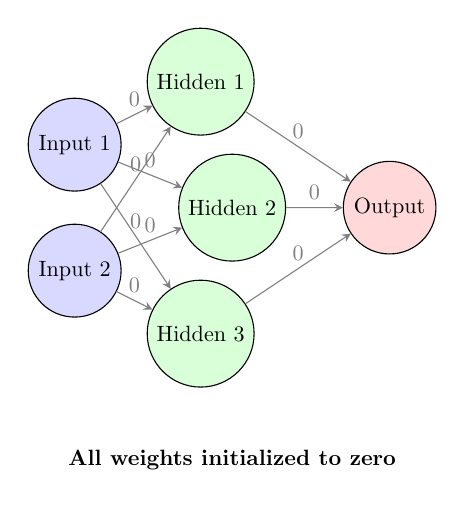
\begin{tikzpicture}[
                node distance=1.0cm, 
                >=stealth, 
                scale=0.8, 
                every node/.style={scale=0.8},
                % Define styles for nodes
                input neuron/.style={circle, draw=black, fill=blue!15, minimum size=0.8cm},
                hidden neuron/.style={circle, draw=black, fill=green!15, minimum size=0.8cm},
                output neuron/.style={circle, draw=black, fill=red!15, minimum size=0.8cm}
            ]
                
                % Define nodes
                \node[input neuron] (I1) at (0,2) {Input 1};
                \node[input neuron] (I2) at (0,0) {Input 2};

                \node[hidden neuron] (H1) at (2,3) {Hidden 1};
                \node[hidden neuron] (H2) at (2.5,1) {Hidden 2};
                \node[hidden neuron] (H3) at (2,-1) {Hidden 3};

                \node[output neuron] (O) at (5,1) {Output};

                % Draw connections with zero weights
                \draw[->, color=gray] (I1) -- (H1) node[midway, above] {0};
                \draw[->, color=gray] (I1) -- (H2) node[midway, above] {0};
                \draw[->, color=gray] (I1) -- (H3) node[midway, above] {0};
                \draw[->, color=gray] (I2) -- (H1) node[midway, above] {0};
                \draw[->, color=gray] (I2) -- (H2) node[midway, above] {0};
                \draw[->, color=gray] (I2) -- (H3) node[midway, above] {0};
                
                \draw[->, color=gray] (H1) -- (O) node[midway, above] {0};
                \draw[->, color=gray] (H2) -- (O) node[midway, above] {0};
                \draw[->, color=gray] (H3) -- (O) node[midway, above] {0};

                % Add annotation below the diagram
                \node[align=center] at (2.5, -3) {\textbf{All weights initialized to zero}};
            \end{tikzpicture}
    \end{columns}

\end{frame}

\begin{frame}{Why Weight Initialization Matters}

    
    \textbf{Importance:}
    \begin{itemize}
        \item Proper initialization ensures faster convergence and improves training stability.
        \item Prevents issues like vanishing or exploding gradients, which can make training slow or unstable.
    \end{itemize}
    
    \textbf{Question:} How can we initialize weights to maximize learning efficiency and prevent gradient problems?
    
\end{frame}

\begin{frame}{Key Initialization Techniques}

    \begin{itemize}
        \item \textbf{Zero Initialization:} Set all weights to zero. 
        \begin{itemize}
            \item Rarely used, as it leads to identical updates for all neurons.
        \end{itemize}
        
        \item \textbf{Random Initialization:} Assign small random values to weights.
        \begin{itemize}
            \item Helps break symmetry, but can still cause issues with gradient magnitudes.
        \end{itemize}
        
        \item \textbf{Xavier Initialization:} 
        \begin{itemize}
            \item Scales weights by \(\sqrt{\frac{1}{\text{number of input neurons}}}\).
            \item Maintains variance across layers for efficient learning, suitable for sigmoid and tanh activations.
        \end{itemize}
        
        \item \textbf{He Initialization:} 
        \begin{itemize}
            \item Scales weights by \(\sqrt{\frac{2}{\text{number of input neurons}}}\).
            \item Optimized for ReLU activation functions to prevent vanishing/exploding gradients.
        \end{itemize}
        
        \item \textbf{Key Point:} Proper initialization reduces the risk of gradient issues and helps the network converge faster.
    \end{itemize}
    
\end{frame}
\begin{frame}{Xavier vs He}
    \begin{center}
        \includegraphics[width=10cm]{pic/Evolution-of-loss-term-for-Xavier-weight-initialization-and-He-weight-initialization.png}  
    \end{center}
Evolution of loss term for Xavier weight initialization and He weight initialization.
\end{frame}
\begin{frame}{Choosing the Right Initialization – Examples}

    \begin{itemize}
        \item \textbf{Scenario 1:} Using ReLU activation functions in a deep network.
        \begin{itemize}
            \item \textbf{Best Choice:} He Initialization.
            \item \textbf{Reason:} Helps maintain gradient flow through the layers.
        \end{itemize}
        
        \item \textbf{Scenario 2:} Using Sigmoid activation functions in a shallow network.
        \begin{itemize}
            \item \textbf{Best Choice:} Xavier Initialization.
            \item \textbf{Reason:} Keeps variance balanced, which is crucial for non-ReLU activations.
        \end{itemize}
        
        \item \textbf{Experiment:} Try initializing with zeros and random weights to see how it impacts training speed and performance.
    \end{itemize}
    
\end{frame}

\begin{frame}{Transition to Loss and Activation Functions}

    \textbf{Recap:} Proper weight initialization:
    \begin{itemize}
        \item Ensures stability during training by maintaining gradient magnitudes.
        \item Helps the network converge faster and learn more effectively.
    \end{itemize}
    
    \textbf{Next Steps:}
    \begin{itemize}
        \item Once weights are initialized, the network needs a measure of error — this is where \textbf{loss functions} come in.
        \item After initializing weights, \textbf{activation functions} determine the output of each neuron, enabling the network to learn complex patterns.
    \end{itemize}
    
    \textbf{Question:} How do we measure the error in predictions and adjust our weights to minimize it?
    
\end{frame}


\subsection{Loss Functions}
\begin{frame}{Overview of Loss Functions}
    \textbf{Types of Loss Functions:}
    \begin{itemize}
        \item \textbf{Mean Squared Error (MSE):} Used in regression to minimize the squared difference between predicted and true values.
        \item \textbf{Mean Absolute Error (MAE):} Also for regression, minimizing absolute differences between predicted and true values.
        \item \textbf{Binary Cross-Entropy:} Used for binary classification to minimize the difference between predicted probabilities and binary labels.
        \item \textbf{Categorical Cross-Entropy:} For multi-class classification, comparing predicted probabilities across multiple classes.
    \end{itemize}
\end{frame}
\begin{frame}{Mean Squared Error (MSE) – Multiple Samples}

    \textbf{Mean Squared Error (MSE):}
    \[
    \text{MSE} = \frac{1}{N} \sum_{i=1}^{N} \left( y_i - \hat{y}_i \right)^2
    \]

    \textbf{Example:}
    \begin{itemize}
        \item Predicted values: \( \hat{y} = [4.2, 3.8, 5.1] \)
        \item True values: \( y = [5.0, 4.0, 4.9] \)
        \item Calculation:
        \[
        \text{MSE} = \frac{1}{3} \left[ (5.0 - 4.2)^2 + (4.0 - 3.8)^2 + (4.9 - 5.1)^2 \right]
        \]
        \[
        \text{MSE} = \frac{1}{3} \left[ 0.64 + 0.04 + 0.04 \right] = \frac{0.72}{3} = 0.24
        \]
    \end{itemize}
\end{frame}

\begin{frame}{Mean Absolute Error (MAE) – Multiple Samples}

    \textbf{Mean Absolute Error (MAE):}
    \[
    \text{MAE} = \frac{1}{N} \sum_{i=1}^{N} \left| y_i - \hat{y}_i \right|
    \]

    \textbf{Example:}
    \begin{itemize}
        \item Predicted values: \( \hat{y} = [4.2, 3.8, 5.1] \)
        \item True values: \( y = [5.0, 4.0, 4.9] \)
        \item Calculation:
        \[
        \text{MAE} = \frac{1}{3} \left( |5.0 - 4.2| + |4.0 - 3.8| + |4.9 - 5.1| \right)
        \]
        \[
        \text{MAE} = \frac{1}{3} (0.8 + 0.2 + 0.2) = \frac{1.2}{3} \approx 0.4
        \]
    \end{itemize}
\end{frame}



\begin{frame}{Binary Classification Loss – Binary Cross-Entropy}

    \textbf{Binary Cross-Entropy:}
    \[
    \mathcal{L}_{\text{BCE}} = -\frac{1}{n} \sum_{i=1}^{n} \left[ y_i \log(\hat{y}_i) + (1 - y_i) \log(1 - \hat{y}_i) \right]
    \]

    \textbf{Example:}
    \begin{itemize}
        \item Predicted probabilities: \( \hat{y} = [0.7, 0.3, 0.9] \)
        \item True labels: \( y = [1, 0, 1] \)
        \item Calculation:
        \[
        \mathcal{L}_{\text{BCE}} = -\frac{1}{3} \left[ \log(0.7) + \log(0.7) + \log(0.9) \right]
        \]
        \[
        \approx -\frac{1}{3} \left( -0.357 + -0.357 + -0.105 \right) \approx 0.273
        \]
    \end{itemize}
    Used to minimize the error between predicted probabilities and binary labels.
    
\end{frame}

\begin{frame}{Multi-Class Classification Loss – Categorical Cross-Entropy}

    \textbf{Categorical Cross-Entropy:}
    \[
    \mathcal{L}_{\text{CCE}} = -\sum_{i=1}^{n} \sum_{c=1}^{C} y_{i,c} \log(\hat{y}_{i,c})
    \]

    \textbf{Example (3-Class):}
    \begin{itemize}
        \item True labels (One-hot): Class 2, Class 1, Class 3
        \item Predicted probabilities:
        \[
        \hat{y} = \left[ [0.1, 0.7, 0.2], [0.6, 0.3, 0.1], [0.1, 0.6, 0.3] \right]
        \]
        \item Calculation:
        \[
        \mathcal{L}_{\text{CCE}} = -\frac{1}{3} \left( \log(0.7) + \log(0.6) + \log(0.3) \right)
        \]
        \[
        \approx -\frac{1}{3} (-0.357 - 0.511 - 1.204) \approx 0.691
        \]
    \end{itemize}
    Optimizes multi-class classification by matching predicted probabilities to true classes.
    
\end{frame}


% \begin{frame}{Loss Functions}
%     \textbf{Types of Loss Functions:}
    
%     \begin{itemize}
%         \item \textbf{Mean Squared Error (MSE):} Commonly used for regression tasks.
%         \[
%         \text{MSE} = \frac{1}{n} \sum_{i=1}^{n} \left( y_i - \hat{y}_i \right)^2
%         \]
%         \item \textbf{Cross-Entropy Loss:} Used for classification tasks.
%         \[
%         \mathcal{L}_{\text{CE}} = -\sum_{i=1}^{n} y_i \log(\hat{y}_i)
%         \]
%     \end{itemize}
%     \vspace{-1cm}
% \begin{center}
% \begin{tikzpicture}[
%     font=\scriptsize,
%     scale=0.9,
%     every node/.style={scale=0.9},
%     neuron/.style={circle, draw=black, thick, minimum size=0.7cm},
%     loss/.style={rectangle, draw=black, thick, minimum size=0.7cm},
%     output/.style={rectangle, draw=black, thick, minimum size=0.7cm},
%     ->, thick
% ]

% % Input
% \node at (0,0) (input) {Input Features};

% % Neural Network
% \node[neuron] at (2.5,0) (neuron) {NN};

% % Output of Neural Network for Regression
% \node[output] at (5,0.7) (pred_reg) {$\hat{y}_{\text{reg}} = 4.2$};
% \node at (7.5,0.7) (true_reg) {$y_{\text{reg}} = 5.0$};

% % Output of Neural Network for Classification
% \node[output] at (5,-1) (pred_class) {$\hat{y}_{\text{class}} = 0.7$};
% \node at (7.5,-1) (true_class) {$y_{\text{class}} = 1$};

% % Loss Function for Regression
% \node[loss] at (10,0.7) (mse) {MSE Loss};

% % Loss Function for Classification
% \node[loss] at (10,-1) (cross_entropy) {Cross-Entropy Loss};

% % Arrows for Regression
% \draw[->] (input) -- (neuron);
% \draw[->] (neuron) -- (pred_reg);
% \draw[->] (pred_reg) -- (true_reg);
% \draw[->] (true_reg) -- (mse);

% % Arrows for Classification
% \draw[->] (neuron) -- (pred_class);
% \draw[->] (pred_class) -- (true_class);
% \draw[->] (true_class) -- (cross_entropy);

% % Labels
% \node at (2.5,1) {Neural Network};
% \node at (10,1.5) {Error Calculation};

% \end{tikzpicture}
% \end{center}

% \end{frame}

% \begin{frame}{Diagram Explanation}
%     \begin{itemize}
               
%         \item \textbf{Regression Prediction:}
%         \begin{itemize}
%             \item Predicted value: \( \hat{y}_{\text{reg}} = 4.2 \) (for example, predicting house price).
%             \item True value: \( y_{\text{reg}} = 5.0 \).
%             \item \textbf{Mean Squared Error (MSE)}:
%             \[
%             \text{MSE} = \frac{1}{n} \sum_{i=1}^{n} (y_i - \hat{y}_i)^2
%             \]
%             \[
%             \text{MSE} = (5.0 - 4.2)^2 = 0.64
%             \]
%             The model needs to minimize this error to improve predictions.
%         \end{itemize}
%     \end{itemize}
%            \begin{itemize}
%         \item \textbf{Classification Prediction:}
%         \begin{itemize}
%             \item Predicted probability: \( \hat{y}_{\text{class}} = 0.7 \) (70\% chance of the input being in class 1).
%             \item True label: \( y_{\text{class}} = 1 \) (the actual class is 1).
%             \item \textbf{Cross-Entropy Loss}:
%             \[
%             \mathcal{L}_{\text{CE}} = - \left( y \log(\hat{y}) \right)
%             \]
%             \[
%             \mathcal{L}_{\text{CE}} = -\left( 1 \cdot \log(0.7) \right) \approx 0.357
%             \]
%             The model needs to minimize this loss to correctly classify inputs.
%         \end{itemize}
%         \end{itemize}
% \end{frame}

% \begin{frame}{Mean Absolute Error (MAE)}
%     \textbf{Mean Absolute Error (MAE):} Commonly used for regression tasks, this loss function measures the average absolute differences between predicted and actual values.

%     \[
%     \text{MAE} = \frac{1}{n} \sum_{i=1}^{n} \left| y_i - \hat{y}_i \right|
%     \]

%     \textbf{Example:}
%     \begin{itemize}
%         \item Predicted value: \( \hat{y}_{\text{reg}} = 4.2 \)
%         \item True value: \( y_{\text{reg}} = 5.0 \)
%         \item \textbf{Calculation:}
%         \[
%         \text{MAE} = \left| 5.0 - 4.2 \right| = 0.8
%         \]
%         The model aims to minimize the MAE to improve the prediction accuracy.
%     \end{itemize}
% \end{frame}

% \begin{frame}{Binary Cross-Entropy Loss}
%     \textbf{Binary Cross-Entropy Loss:} Used for binary classification tasks where the output is either 0 or 1. It measures the difference between predicted and true binary labels.

%     \[
%     \mathcal{L}_{\text{BCE}} = -\frac{1}{n} \sum_{i=1}^{n} \left[ y_i \log(\hat{y}_i) + (1 - y_i) \log(1 - \hat{y}_i) \right]
%     \]

%     \textbf{Example:}
%     \begin{itemize}
%         \item Predicted probability: \( \hat{y} = 0.7 \) (70\% chance of being class 1)
%         \item True label: \( y = 1 \)
%         \item \textbf{Calculation:}
%         \[
%         \mathcal{L}_{\text{BCE}} = - \left( 1 \cdot \log(0.7) + 0 \cdot \log(0.3) \right) \approx 0.357
%         \]
%         The model minimizes this loss to correctly classify binary outputs.
%     \end{itemize}
% \end{frame}

% \begin{frame}{Categorical Cross-Entropy Loss (Multi-Class)}
%     \textbf{Categorical Cross-Entropy Loss:} Used for multi-class classification tasks where each output corresponds to a class. It measures the difference between the predicted probabilities and the true class labels.

%     \[
%     \mathcal{L}_{\text{CCE}} = -\sum_{i=1}^{n} \sum_{c=1}^{C} y_{i,c} \log(\hat{y}_{i,c})
%     \]

%     \textbf{Example (3-class Classification):}
%     \begin{itemize}
%         \item True label: Class 2 (One-hot encoded as [0, 1, 0])
%         \item Predicted probabilities: [0.1, 0.7, 0.2]
%         \item \textbf{Calculation:}
%         \[
%         \mathcal{L}_{\text{CCE}} = -\left( 0 \cdot \log(0.1) + 1 \cdot \log(0.7) + 0 \cdot \log(0.2) \right)
%         \]
%         \[
%         \approx -\log(0.7) \approx 0.357
%         \]
%         The model minimizes this loss to accurately predict multi-class outputs.
%     \end{itemize}
% \end{frame}


\subsection{Activation Functions}
\begin{frame}{Linear Activation - A Limitation}
    \textbf{Linear Activation:} 
    \[
    f(z) = z
    \]
    
    \begin{itemize}
        \item Example: If a neuron produces a raw output \( z = 5.7 \), linear activation would pass this unchanged.
    \end{itemize}
    
    % Start of TikZ Diagram
    \begin{center}
    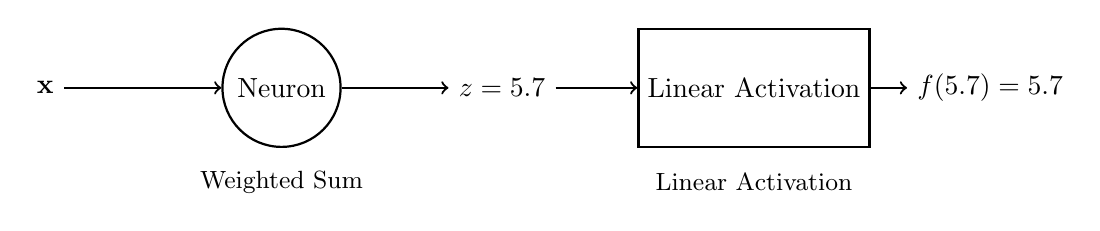
\begin{tikzpicture}[
        neuron/.style={circle, draw=black, thick, minimum size=1.5cm},
        activation/.style={rectangle, draw=black, thick, minimum size=1.5cm},
        ->, thick
    ]
    
    % Input
    \node at (0,0) (input) {$\mathbf{x}$};
    
    % Neuron
    \node[neuron] at (3,0) (neuron) {Neuron};
    
    % Output of Neuron
    \node at (5.8,0) (raw) {$z = 5.7$};
    
    % Linear Activation Box
    \node[activation] at (9,0) (activation) {Linear Activation};
    
    % Final Output
    \node at (12,0) (output) {$f(5.7) = 5.7$};
    
    % Arrows
    \draw[->] (input) -- (neuron);
    \draw[->] (neuron) -- (raw);
    \draw[->] (raw) -- (activation);
    \draw[->] (activation) -- (output);
    
    % Labels
    \node at (3, -1.2) {\small Weighted Sum};
    \node at (9, -1.2) {\small Linear Activation};
    
    \end{tikzpicture}
    \end{center}
    
\end{frame}


\begin{frame}{Limitation of Linear Activation}

    \textbf{Why Transform Outputs?} Raw outputs need to be transformed into meaningful values, such as probabilities.

    \textbf{The Problem:} Linear activation lacks non-linearity, restricting the model to simple linear relationships.
\end{frame}
%%%%%%%%%%%%%%%%%%%%%%%%%%%%%%%%%%%%%%%%%%% act %%%%%%%%%%%%%%%%%%%%%%%%%%%%%%%%%%%%%%%


\begin{frame}
    \frametitle{Sigmoid}

    \textbf{Characteristics of Sigmoid:}
    \begin{equation*}
              \sigma(z) = \frac{1}{1 + e^{-z}}
    \end{equation*}
    \begin{itemize}
        \item Squashes the input between 0 and 1, which makes it useful in probabilistic interpretations (e.g., logistic regression).
        \item Often used in output layers for binary classification problems.
    \end{itemize}

    \begin{center}
    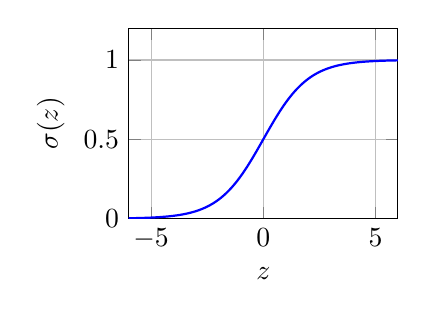
\begin{tikzpicture}
        % Sigmoid function plot
        \begin{axis}[
            width=5cm, height=4cm,
            xlabel={$z$}, ylabel={$\sigma(z)$},
            grid=major, xmin=-6, xmax=6, ymin=0, ymax=1.2
        ]
        \addplot[color=blue, thick, domain=-6:6, samples=100] {1/(1+exp(-x))};
        \end{axis}
    \end{tikzpicture}
    \end{center}
\end{frame}

\begin{frame}
    \frametitle{Model: Sigmoid Decision Surface}

        \begin{figure}
        \centering
        \includegraphics[width=0.8\textwidth]{pic/sig.png}  
    \end{figure}
\end{frame}

\begin{frame}{Classification: Tumor Detection (Malignant vs. Benign)}
    \textbf{Sigmoid Activation:} Useful for binary classification!
    
    \begin{itemize}
        \item Example: For \( z = 5.7 \),
        \[
        \sigma(5.7) \approx 0.9966
        \]
    \end{itemize}
    \vspace{-8mm}
    % Start of TikZ Diagram
    \begin{center}
    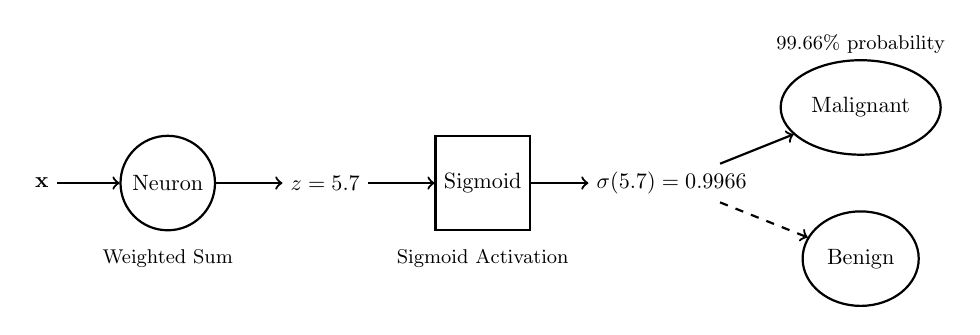
\begin{tikzpicture}[
         scale=0.8,
         every node/.style={scale=0.8},
        neuron/.style={circle, draw=black, thick, minimum size=1.5cm},
        activation/.style={rectangle, draw=black, thick, minimum size=1.5cm},
        decision/.style={ellipse, draw=black, thick, minimum size=1.5cm},
        ->, thick
    ]
    
    % Input
    \node at (2,0) (input) {$\mathbf{x}$};
    
    % Neuron
    \node[neuron] at (4,0) (neuron) {Neuron};
    
    % Raw Output of Neuron
    \node at (6.5,0) (raw) {$z = 5.7$};
    
    % Sigmoid Activation Box
    \node[activation] at (9,0) (activation) {Sigmoid};
    
    % Sigmoid Output
    \node at (12,0) (prob) {$\sigma(5.7) = 0.9966$};
    
    % Classification Decision: Malignant vs. Benign
    \node[decision] at (15,1.2) (malignant) {Malignant};
    \node[decision] at (15,-1.2) (benign) {Benign};
    
    % Arrows
    \draw[->] (input) -- (neuron);
    \draw[->] (neuron) -- (raw);
    \draw[->] (raw) -- (activation);
    \draw[->] (activation) -- (prob);
    
    % Probability-based decision arrows
    \draw[->] (prob) -- (malignant);
    \draw[->, dashed] (prob) -- (benign);
    
    % Labels
    \node at (4, -1.2) {\small Weighted Sum};
    \node at (9, -1.2) {\small Sigmoid Activation};
    \node at (15, 2.2) {\small 99.66\% probability};
    
    \end{tikzpicture}
    \end{center}
    
\end{frame}

\begin{frame}{Sigmoid}
    \textbf{Limitations of Sigmoid:}
    \begin{itemize}
        \item \textbf{Gradient Saturation:} When \( z \) is very large or very small, the gradient becomes nearly zero, causing slow learning (vanishing gradient problem).
        \item \textbf{Not Zero-Centered:} The output is not zero-centered, which can make optimization more difficult.
    \end{itemize}

    \textbf{Question:}
    \begin{itemize}
        \item Why does the vanishing gradient problem occur with Sigmoid during backpropagation? (To be discussed in more detail later)
    \end{itemize}
\end{frame}


\begin{frame}{Problem: Multi-Class Tumor Classification}
    \textbf{Scenario:} We want to classify a tumor into one of three categories:
    \begin{itemize}
        \item \textbf{Class 0}: Benign
        \item \textbf{Class 1}: Malignant
        \item \textbf{Class 2}: Pre-cancerous
    \end{itemize}
    
    \textbf{Goal:} Given a set of tumor features, predict which class the tumor belongs to.
    
    This is a \textbf{multi-class classification problem}, and we will use the \textbf{Softmax activation function} to assign probabilities to each class.
    
            \begin{figure}
\centerline{\includegraphics[scale=.4]{pic/cancer.jpg}}

\label{fig}
\end{figure}
\end{frame}
\begin{frame}{Softmax Activation: The Model}
    In multi-class classification, Softmax is used to convert raw outputs (logits) into probabilities for each class.
    
    \textbf{Softmax Function:}
    \[
    P(y = i | X) = \frac{e^{z_i}}{\sum_{j=1}^{K} e^{z_j}}
    \]
    Where:
    \begin{itemize}
        \item \( z_i \) is the raw output (logit) for class \( i \).
        \item \( K \) is the number of classes (in this case, 3: benign, malignant, pre-cancerous).
    \end{itemize}
    
    The Softmax function ensures that the sum of the probabilities for all classes is 1, and the class with the highest probability is chosen as the prediction.
\end{frame}

\begin{frame}{Example: Softmax Calculation}
    Consider a tumor with the following logits from a neural network:
    \begin{itemize}
        \item Logit for Benign (Class 0): \( z_0 = 1.5 \)
        \item Logit for Malignant (Class 1): \( z_1 = 0.8 \)
        \item Logit for Pre-Cancerous (Class 2): \( z_2 = -0.5 \)
    \end{itemize}
    
    \textbf{Step 1: Exponentiate the logits}
    \[
    e^{z_0} = e^{1.5} \approx 4.48, \quad e^{z_1} = e^{0.8} \approx 2.23, \quad e^{z_2} = e^{-0.5} \approx 0.61
    \]
    
    \textbf{Step 2: Compute the sum of exponentials}
    \[
    \text{Sum} = e^{z_0} + e^{z_1} + e^{z_2} = 4.48 + 2.23 + 0.61 = 7.32
    \]
\end{frame}

\begin{frame}{Example: Softmax Probabilities}
    \textbf{Step 3: Calculate Softmax probabilities for each class}
    \[
    P(\text{Benign}) = \frac{4.48}{7.32} \approx 0.612, \quad P(\text{Malignant}) = \frac{2.23}{7.32} \approx 0.305, \quad P(\text{Pre-Cancerous}) = \frac{0.61}{7.32} \approx 0.083
    \]
    
    \textbf{Step 4: Make a classification decision}
    \begin{itemize}
        \item The highest probability is \( 0.612 \) for the \textbf{Benign} class.
        \item Therefore, the model predicts that the tumor is \textbf{Benign} (Class 0).
    \end{itemize}
\end{frame}

\begin{frame}{Conclusion: Softmax Activation for Classification}
    \textbf{Key Points:}
    \begin{itemize}
        \item Softmax is used in the output layer for \textbf{multi-class classification}.
        \item It converts logits into a \textbf{probability distribution} across classes.
        \item The class with the highest probability is selected as the prediction.
    \end{itemize}
    
    \textbf{Main Idea:} Softmax ensures all outputs sum to 1, making it ideal for choosing one class out of multiple options.
\end{frame}



\begin{frame}
    \frametitle{Tanh (Hyperbolic Tangent)}

    \textbf{Characteristics of Tanh:}
    \begin{equation*}
        \tanh(z) = \frac{e^z - e^{-z}}{e^z + e^{-z}}
    \end{equation*}
    \begin{itemize}
        \item Squashes input between -1 and 1, making it zero-centered (Balanced Updates $\rightarrow$ Reduced Bias in Gradient Descent $\rightarrow$ Faster Convergence)
    \end{itemize}

    \textbf{Advantages of Tanh:}
    \begin{itemize}
        \item \textbf{Zero-Centered}: Output ranges from -1 to 1, making optimization easier.
        \item Better for \textbf{hidden layers} than Sigmoid due to zero-centered output.
    \end{itemize}

    \textbf{Limitations:}
    \begin{itemize}
        \item Similar saturation issues as Sigmoid: large input values push gradients towards zero (vanishing gradient problem).
    \end{itemize}

\end{frame}

\begin{frame}{Tanh (Hyperbolic Tangent)}
     \begin{center}
    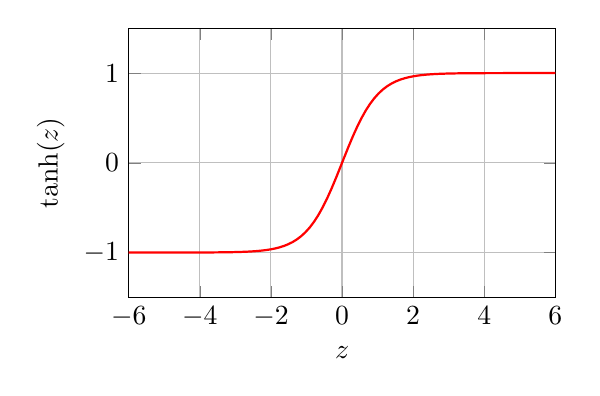
\begin{tikzpicture}
        % Tanh function plot
        \begin{axis}[
            width=7cm, height=5cm,
            xlabel={$z$}, ylabel={$\tanh(z)$},
            grid=major, xmin=-6, xmax=6, ymin=-1.5, ymax=1.5
        ]
        \addplot[color=red, thick, domain=-6:6, samples=100] {tanh(x)};
        \end{axis}
    \end{tikzpicture}
    \end{center}

    \textbf{Question:}
    \begin{itemize}
        \item How does Tanh help with faster convergence compared to Sigmoid?
    \end{itemize}   
\end{frame}
\begin{frame}{Comparison: Sigmoid vs Tanh}
    \centering
    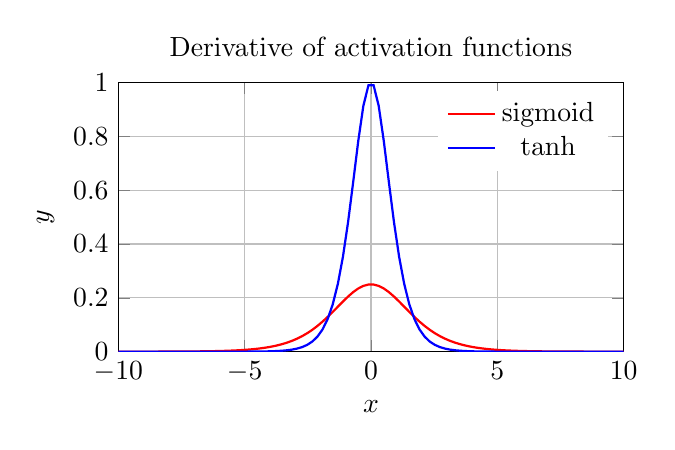
\begin{tikzpicture}
    \begin{axis}[
        width=8cm, height=5cm,
        xlabel={$x$}, ylabel={$y$},
        title={Derivative of activation functions},
        grid=major,
        xmin=-10, xmax=10, ymin=0, ymax=1,
        legend pos=north east,
        legend style={draw=none},
    ]
    
    % Sigmoid derivative plot
    \addplot[color=red, thick] 
        plot[domain=-10:10, samples=100] 
        {exp(-x)/(1+exp(-x))^2};
    \addlegendentry{sigmoid}
    
    % Tanh derivative plot
    \addplot[color=blue, thick] 
        plot[domain=-10:10, samples=100] 
        {1 - tanh(x)^2};
    \addlegendentry{tanh}
    
    \end{axis}
\end{tikzpicture}
\begin{itemize}
    \item The derivative of the Tanh function has a much steeper slope at $x=0$, meaning it provides a larger gradient for backpropagation compared to the Sigmoid function.
\end{itemize}

\end{frame}
\begin{frame}
    \frametitle{Comparison: Sigmoid vs Tanh}

    \textbf{Key Differences:}
    \begin{itemize}
        \item \textbf{Sigmoid}: Maps input to [0, 1]. Output is not zero-centered.
        \item \textbf{Tanh}: Maps input to [-1, 1]. Output is zero-centered, leading to easier optimization.
    \end{itemize}

    \begin{center}
    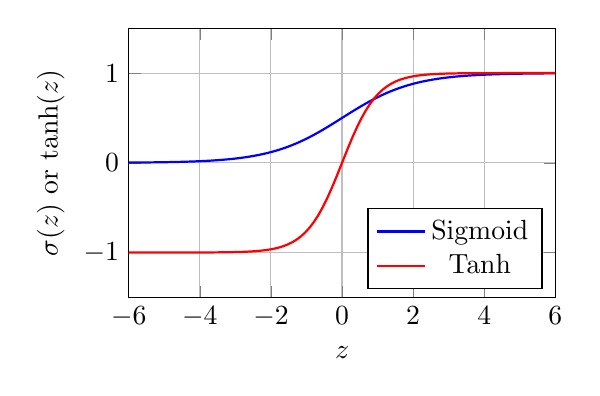
\begin{tikzpicture}
        % Comparison of Sigmoid and Tanh
        \begin{axis}[
            width=7cm, height=5cm,
            xlabel={$z$}, ylabel={$\sigma(z)$ or $\tanh(z)$},
            grid=major, xmin=-6, xmax=6, ymin=-1.5, ymax=1.5,
            legend pos=south east
        ]
        \addplot[color=blue, thick, domain=-6:6, samples=100] {1/(1+exp(-x))};
        \addlegendentry{Sigmoid}
        \addplot[color=red, thick, domain=-6:6, samples=100] {tanh(x)};
        \addlegendentry{Tanh}
        \end{axis}
    \end{tikzpicture}
    \end{center}

\end{frame}
\begin{frame}{Comparison: Sigmoid vs Tanh}
        \textbf{When to Use:}
    \begin{itemize}
        \item \textbf{Sigmoid}: Best for binary classification tasks, particularly in the output layer.
        \item \textbf{Tanh}: More suitable for hidden layers due to its centered output, allowing faster training.
    \end{itemize}
    \textbf{Question:}
    \begin{itemize}
        \item In what scenario might Sigmoid be preferred over Tanh, despite its limitations?
    \end{itemize}
\end{frame}
\begin{frame}{Neural Networks: Why is the Max Operator Important?}
  \begin{itemize}
      \item \textbf{Before:} Linear score function:
      \[
      f = Wx
      \]
      \item \textbf{Now:} 2-layer Neural Network:
      \[
      f = W_2 \max(0, W_1 x)
      \]
      \item The function \(\max(0, z)\) is called an activation function (in this case, ReLU).
      \item \textcolor{red}{Q: What if we try to build a neural network without an activation function?}
      \[
      f = W_2 W_1 x
      \]
      \[
      W_3 = W_2 W_1 \in \mathbb{R}^{C \times H}, \quad f = W_3 x
      \]
      \item \textbf{A:} We end up with a linear classifier again!
  \end{itemize}
\end{frame}

\begin{frame}
    \frametitle{ReLU}
    \textbf{Characteristics of ReLU:}
     \begin{equation*}
      \text{ReLU}(z) = \max(0, z) 
       \end{equation*}
       \begin{itemize}
           \item Faster convergence: Efficient computation, especially for deep networks.
       \end{itemize}
    \textbf{Advantages of ReLU:}
    \begin{itemize}
        \item Does not saturate for positive values, helping to avoid the vanishing gradient problem.
        \item Computationally efficient (simpler than Sigmoid/Tanh).
    \end{itemize}

    \begin{center}
    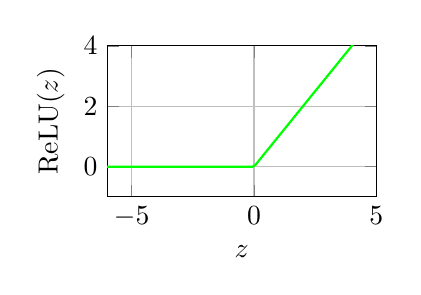
\begin{tikzpicture}
        % ReLU function plot
        \begin{axis}[
            width=5cm, height=3.5cm,
            xlabel={$z$}, ylabel={ReLU($z$)},
            grid=major, xmin=-6, xmax=5, ymin=-1, ymax=4
        ]
        \addplot[color=green, thick, domain=-6:6, samples=100] {max(0, x)};
        \end{axis}
    \end{tikzpicture}
    \end{center}
\end{frame}
\begin{frame}{ReLU}

    \textbf{Limitation:}
    \begin{itemize}
        \item \textbf{Dead ReLU Problem}: Neurons can become inactive during training, outputting 0 for all inputs if they receive negative values consistently.
    \end{itemize}

    \textbf{Question:}
    \begin{itemize}
        \item Why does ReLU lead to faster training in deep networks?
    \end{itemize}

\end{frame}

\begin{frame}
    \frametitle{Variants of ReLU: Leaky ReLU, PReLU, ELU}
    \centering
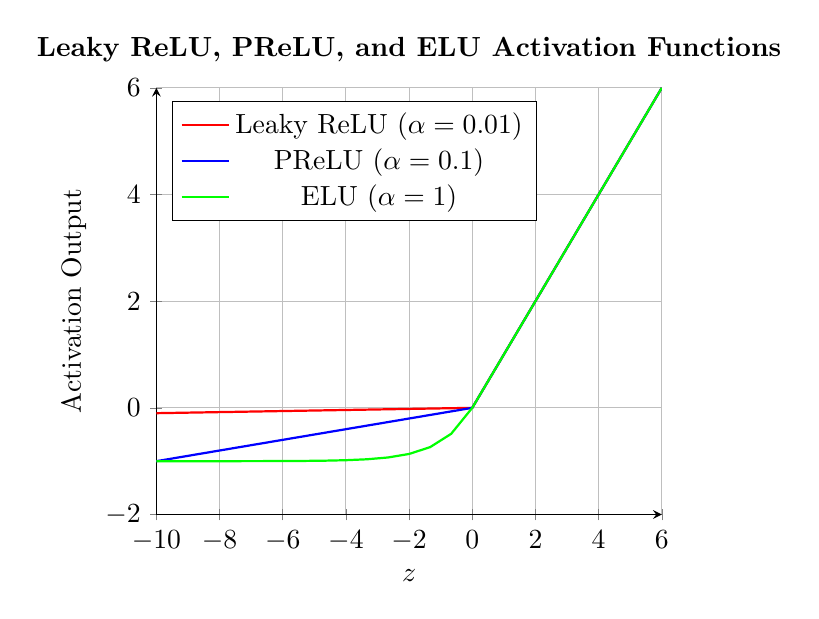
\begin{tikzpicture}
    \begin{axis}[
        width=8cm, height=7cm,
        xlabel={$z$}, ylabel={Activation Output},
        grid=major,
        xmin=-10, xmax=6, ymin=-2, ymax=6,
        legend pos=north west,
        title={\textbf{Leaky ReLU, PReLU, and ELU Activation Functions}},
        axis lines=left,
    ]

    % Leaky ReLU plot (alpha = 0.01)
    \addplot[color=red, thick, domain=-10:6] {max(0.01*x, x)};
    \addlegendentry{Leaky ReLU ($\alpha = 0.01$)}

    % PReLU plot (alpha = 0.1)
    \addplot[color=blue, thick, domain=-10:6] {max(0.1*x, x)};
    \addlegendentry{PReLU ($\alpha = 0.1$)}

    % ELU plot (alpha = 1)
    \addplot[color=green, thick, domain=-10:6] {x > 0 ? x : (exp(x) - 1)};
    \addlegendentry{ELU ($\alpha = 1$)}

    \end{axis}
\end{tikzpicture}

    
\end{frame}
\begin{frame}
    \frametitle{Variants of ReLU: Leaky ReLU}
    \begin{itemize}
        \item Allows a small, non-zero gradient for negative inputs.
        \begin{equation*}
            \text{LeakyReLU}(z) = \max(\alpha z, z), \quad \alpha = 0.01
        \end{equation*}
        \item Helps prevent the "dead ReLU" problem, where neurons stop updating.
    \end{itemize}
            \begin{center}
            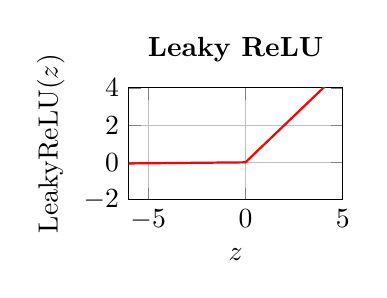
\begin{tikzpicture}
                \begin{axis}[
                    width=4.3cm, height=3cm,
                    xlabel={$z$}, ylabel={LeakyReLU($z$)},
                    grid=major, xmin=-6, xmax=5, ymin=-2, ymax=4,
                    title={\textbf{Leaky ReLU}},
                ]
                \addplot[color=red, thick, domain=-6:6] {max(0.01*x, x)};
                \end{axis}
            \end{tikzpicture}
            \end{center}
            \centering
            \textbf{Leaky ReLU:} Allows a small, non-zero gradient for negative inputs.
\end{frame}
\begin{frame}{Variants of ReLU: PReLU (Parametric ReLU)}
    \begin{itemize}
        \item Similar to Leaky ReLU, but the slope for negative inputs (\( \alpha \)) is learned during training.
        \begin{equation*}
            \text{PReLU}(z) = \max(\alpha z, z), \quad \alpha \text{ is learned}
        \end{equation*}
        \item Provides more flexibility by adjusting the slope for negative inputs based on data.
    \end{itemize} 
        %     % PReLU Diagram
            \begin{center}
            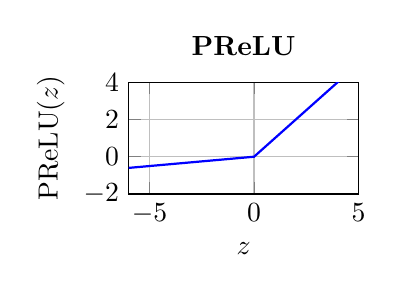
\begin{tikzpicture}
                \begin{axis}[
                    width=4.5cm, height=3cm,
                    xlabel={$z$}, ylabel={PReLU($z$)},
                    grid=major, xmin=-6, xmax=5, ymin=-2, ymax=4,
                    title={\textbf{PReLU}},
                ]
                \addplot[color=blue, thick, domain=-6:6] {max(0.1*x, x)};
                \end{axis}
            \end{tikzpicture}
            \end{center}
            \centering
            \textbf{PReLU:} Similar to Leaky ReLU, with a learnable slope.
\end{frame}
\begin{frame}{Variants of ReLU: ELU (Exponential Linear Unit)}
    \begin{itemize}
        \item Similar to ReLU for positive values but smoother for negative inputs.
        \begin{equation*}
            \text{ELU}(z) =
            \begin{cases}
                z, & \text{if } z > 0 \\
                \alpha (e^z - 1), & \text{if } z \leq 0
            \end{cases}, \quad \alpha = 1
        \end{equation*}
        \item Provides faster convergence and reduces bias shift by smoothing negative values.
    \end{itemize}
                \begin{center}
            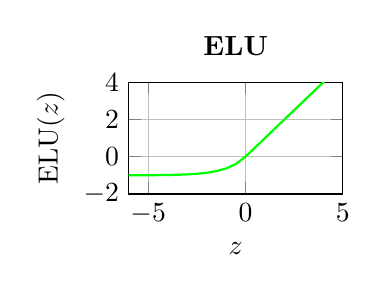
\begin{tikzpicture}
                \begin{axis}[
                    width=4.3cm, height=3cm,
                    xlabel={$z$}, ylabel={ELU($z$)},
                    grid=major, xmin=-6, xmax=5, ymin=-2, ymax=4,
                    title={\textbf{ELU}},
                ]
                \addplot[color=green, thick, domain=-6:6] {x > 0 ? x : (exp(x) - 1)};
                \end{axis}
            \end{tikzpicture}
            \end{center}
            \vspace{-0.3cm}
            \centering
            \textbf{ELU:} Smoother than ReLU for negative values.
\end{frame}

%%%%%%%%%%%%%%%%%%%%%%%%%%%%%%%%%%%%%%%%%%% act %%%%%%%%%%%%%%%%%%%%%%%%%%%%%%%%%%%%%%%




\section{References}
\begin{frame}[allowframebreaks]
    \bibliography{ref}
    \bibliographystyle{ieeetr}
    \nocite{*} % used here because no citation happens in slides
    % if there are too many try use:
    % \tiny\bibliographystyle{alpha}
\end{frame}


\begin{frame}
    \begin{center}
        {\Huge Any Questions?}
    \end{center}
\end{frame}

\end{document}
